\documentclass[conference]{IEEEtran}
\IEEEoverridecommandlockouts
% The preceding line is only needed to identify funding in the first footnote. If that is unneeded, please comment it out.

\usepackage{hyperref}

% --- Tickz
\usepackage{physics}
\usepackage{tikz}
\usepackage{amsmath}
\usepackage{mathdots}
% \usepackage{yhmath}
\usepackage{cancel}
\usepackage{color}
\usepackage{siunitx}
\usepackage{array}
\usepackage{multirow}
% \usepackage{amssymb}
\usepackage{gensymb}
\usepackage{tabularx}
\usepackage{extarrows}
\usepackage{booktabs}
\usetikzlibrary{fadings}
\usetikzlibrary{patterns}
\usetikzlibrary{shadows.blur}
\usetikzlibrary{shapes}

% ---------

\usepackage{balance} % for balancing columns on the final page
\usepackage{csquotes}
% \usepackage{cite}
\newcommand{\probP}{\text{I\kern-0.15em P}}
\usepackage{etoolbox}
\patchcmd{\thebibliography}{\section*{\refname}}{}{}{}
% \usepackage{amsthm,amssymb,amsfonts}

\usepackage[T1]{fontenc}
\usepackage{graphicx}
\usepackage{color}
% \renewcommand\UrlFont{\color{blue}\rmfamily}

\usepackage[inline, shortlabels]{enumitem}
\usepackage{tabularx}
\usepackage{caption}
\usepackage{listings}
\usepackage{stfloats}
\usepackage{titlesec}
\usepackage{amssymb}
\usepackage{amsmath}
\usepackage{ragged2e}
% \usepackage[hyphens]{url}
\usepackage[linesnumbered,ruled,vlined]{algorithm2e}
\usepackage{float}
\usepackage[english]{babel}
\addto\extrasenglish{  
    \def\figureautorefname{Figure}
    \def\tableautorefname{Table}
    \def\algorithmautorefname{Algorithm}
    \def\sectionautorefname{Section}
    \def\subsectionautorefname{Subsection}
    \def\proofoutlineautorefname{Proof Outline}
}

% --------------
\titleclass{\subsubsubsection}{straight}[\subsection]

\newcounter{subsubsubsection}[subsubsection]
\renewcommand\thesubsubsubsection{\thesubsubsection.\arabic{subsubsubsection}}
\renewcommand\theparagraph{\thesubsubsubsection.\arabic{paragraph}} % optional; useful if paragraphs are to be numbered

\titleformat{\subsubsubsection}
  {\normalfont\normalsize\bfseries}{\thesubsubsubsection}{1em}{}
\titlespacing*{\subsubsubsection}
{0pt}{3.25ex plus 1ex minus .2ex}{1.5ex plus .2ex}

\makeatletter
\renewcommand\paragraph{\@startsection{paragraph}{5}{\z@}%
  {3.25ex \@plus1ex \@minus.2ex}%
  {-1em}%
  {\normalfont\normalsize\bfseries}}
\renewcommand\subparagraph{\@startsection{subparagraph}{6}{\parindent}%
  {3.25ex \@plus1ex \@minus .2ex}%
  {-1em}%
  {\normalfont\normalsize\bfseries}}
\def\toclevel@subsubsubsection{4}
\def\toclevel@paragraph{5}
\def\toclevel@paragraph{6}
\def\l@subsubsubsection{\@dottedtocline{4}{7em}{4em}}
\def\l@paragraph{\@dottedtocline{5}{10em}{5em}}
\def\l@subparagraph{\@dottedtocline{6}{14em}{6em}}
\makeatother

\setcounter{secnumdepth}{4}
\setcounter{tocdepth}{4}


\setboolean{@twoside}{false}

% --------------


\newcommand{\before}[1]{\textcolor{red}{#1}}
\newcommand{\after}[1]{\textcolor{green}{#1}}

\newcommand{\old}[1]{\textcolor{orange}{#1}}
\newcommand{\rem}[1]{\textcolor{red}{#1}}
\newcommand{\todo}[1]{\textcolor{orange}{\newline \textit{\textbf{TODO:} #1}} \newline \newline }

\makeatletter
\newcommand{\linebreakand}{%
  \end{@IEEEauthorhalign}
  \hfill\mbox{}\par
  \mbox{}\hfill\begin{@IEEEauthorhalign}
}
\makeatother




% ---------------------------


\begin{document}

\title{Enhancing Explainability and Control in Multi-Agent Reinforcement Learning: A Systems Engineering Approach}

% \IEEEaftertitletext{\vspace{-1\baselineskip}}

\author{

    \IEEEauthorblockN{Julien Soulé}
    \IEEEauthorblockA{\textit{Thales Land and Air Systems, BU IAS}}
    %Rennes, France \\
    \IEEEauthorblockA{\textit{Univ. Grenoble Alpes,} \\
        \textit{Grenoble INP, LCIS, 26000,}\\
        Valence, France \\
        julien.soule@lcis.grenoble-inp.fr}

    \and

    \IEEEauthorblockN{Jean-Paul Jamont\IEEEauthorrefmark{1}, Michel Occello\IEEEauthorrefmark{2}}
    \IEEEauthorblockA{\textit{Univ. Grenoble Alpes,} \\
        \textit{Grenoble INP, LCIS, 26000,}\\
        Valence, France \\
        \{\IEEEauthorrefmark{1}jean-paul.jamont,\IEEEauthorrefmark{2}michel.occello\}@lcis.grenoble-inp.fr
    }

    % \and

    % \IEEEauthorblockN{Michel Occello}
    % \IEEEauthorblockA{\textit{Univ. Grenoble Alpes,} \\
    % \textit{Grenoble INP, LCIS, 26000,}\\
    % Valence, France \\
    % michel.occello@lcis.grenoble-inp.fr}

    % \and

    \linebreakand

    \hspace{-0.5cm}
    \IEEEauthorblockN{Paul Théron}
    \IEEEauthorblockA{
        \hspace{-0.5cm}
        \textit{AICA IWG} \\
        \hspace{-0.5cm}
        La Guillermie, France \\
        \hspace{-0.5cm}
        %lieu-dit Le Bourg, France \\
        paul.theron@orange.fr}

    \and

    \hspace{0.5cm}
    \IEEEauthorblockN{Louis-Marie Traonouez}
    \IEEEauthorblockA{
        \hspace{0.5cm}
        \textit{Thales Land and Air Systems, BU IAS} \\
        \hspace{0.5cm}
        Rennes, France \\
        \hspace{0.5cm}
        louis-marie.traonouez@thalesgroup.com}}


\maketitle

\begin{abstract}
    Multi-Agent Reinforcement Learning (MARL) enables the development of autonomous agent behaviors that adaptively optimize collective performance. However, the lack of explicit organizational constraints limits explainability and control, hindering deployment in critical systems. To address this, we propose MOISE+MARL, a framework that integrates the $\mathcal{M}OISE^+$ organizational model into MARL. By structuring training around predefined roles and goals, our approach enhances both interpretability and policy enforcement, ensuring that agents adhere to organizational specifications. Furthermore, we introduce a post-training trajectory-based analysis method to infer implicit roles and goals, enabling a comprehensive evaluation of agent behaviors. 
    We validate MOISE+MARL across multiple MARL environments and training paradigms, demonstrating its effectiveness in improving stability, scalability, and policy alignment with predefined organizational constraints. Results show that our approach reduces policy variability by up to 40\% while improving organizational fit by 44\%.
    

\end{abstract}

\begin{IEEEkeywords}
    Multi-Agent Reinforcement Learning, Organizational Explainability, Organizational Control
\end{IEEEkeywords}

\section{Introduction}

% Context
Multi-Agent Reinforcement Learning (MARL) enables the discovery of a joint policy that controls agents' behaviors so they can achieve a global goal within a specific environment. 
This joint policy not only dictates the individual actions of agents but also manages their interactions with one another, and potentially with all other agents, without any preconceived notion of a predefined organizational order or structure.

In environments that require social interaction among agents to optimally achieve the global goal, agents may converge in such a way that they exhibit recurring sets of similar behaviors across different testing episodes. 
These distinct sets of behaviors can demonstrate properties of specialization, complementarity, and stability, making them akin to implicit roles~\cite{wilson2008learning, yang2021role}. 
Moreover, the trajectories of agents assuming these "abstract" roles may display similarities, such as recurrent observations at the end of each episode. 
These recurring parts of trajectories can be interpreted as "abstract" goals, suggesting that agents may aim to pursue these as intermediate objectives before reaching the global goal. 
These abstract roles and abstract goals form the foundation of an "abstract" structural and functional organization~\cite{foerster2018counterfactual, liu2021efficient}.

However, it would be misleading to assume that all trained agents in any environment can be faithfully compared to a structural and functional organization. 
Indeed, we can interpret the behaviors of trained agents concerning their similarity to the potential vision of an abstract structural and functional organization, which we define as \textbf{organizational fit}~\cite{berenji2000learning, serrino2019finding}. 
While evaluating organizational fit would be useful to assess to what extent trained agents can naturally be explained as roles and goals, one could also consider the reverse approach. 
By guiding or encouraging agents to converge towards structural and functional organizations with higher organizational fit, we aim to enhance explainability and control in MARL~\cite{van2018explainable, alshiekh2018safe}.

\

% Problem
Building on these assumptions, this paper aims to further explore two key aspects:
\begin{enumerate*}[label={\roman*)}]
    \item The \textbf{evaluation of organizational fit}, which seeks to measure how closely a joint policy aligns with a structural and functional organization. 
    A significant challenge here is to understand under what conditions agents can be considered to form a structural and functional organization, given constraints imposed by the environment, objectives, and other optional factors.
    Existing literature often addresses policy evaluation in terms of roles or goals~\cite{yang2021role, foerster2018communication}, but these works generally lack a systematic and comprehensive approach. 
    Current methods offer few clear tools for quantitatively and qualitatively measuring this organizational fit.
    
    \item The \textbf{control of organizational fit}, which aims to guide agents towards policies that conform to a structural and functional organization through user-defined constraints or incentives that implement roles and goals.
    The primary challenges include reducing the policy search space, improving convergence, and ensuring compliance with safety constraints~\cite{borsa2019constrained, garcia2015comprehensive}.
    Existing approaches in this field often fall short in terms of enabling users to easily define and manage the application of organizational specifications in a practical and flexible manner within a standard MARL framework, without relying on alternative paradigms such as Hierarchical Reinforcement Learning (HRL)~\cite{ghavamzadeh2006cooperative, hi_marl_reference}.
\end{enumerate*}

\

% Contribution
\noindent We introduce the \textbf{MOISE+MARL} framework, which integrates the Decentralized Partially Observable Markov Decision Process (Dec-POMDP) MARL framework with the $\mathcal{M}OISE^+$~\cite{Hubner2007} organizational model through proposed relationships. 
This framework allows users to manually define the logic of a role or a goal by relying on trajectory-based patterns to describe the expected behavior of an agent that has adopted a goal or mission. 
Once configured, they allow users to apply a role to an agent, adding constraints that automatically influence agents' policies by dynamically updating both the action space and reshaping the reward function.
This framework also includes a method called \textbf{Trajectory-based Evaluation in MOISE+MARL} (TEMM), which uses unsupervised learning techniques to generalize abstract roles and abstract missions from observed trajectories across multiple test episodes. 
By measuring the gap between inferred abstract organizational specifications and actual behaviors, this method allows for a quantitative assessment of organizational fit.

\

% Evaluation & Findings
We evaluated the MOISE+MARL framework in the following scenarios:
\begin{enumerate*}[label={\roman*) },itemjoin={; \quad}]
  \item Four distinct environments, each expected to result in the training of joint policies with different abstract organizations, to assess the generalizability of MOISE+MARL's applicability~\cite{rashid2018qmix, overcookedai}
  \item Four MARL algorithms from several families to assess their suitability with MOISE+MARL during training and post-analysis~\cite{yu2021mappo, lowe2017multi}
  \item Four sets of organizational specifications as Policy-Based Decision Trees (PBDTs), one for each environment, to constrain agents in a manner that either enforces conformity intended for both manual and quantitative evaluation.
\end{enumerate*}

In all environments, we observed that agents having adopted roles behave as expected according to their roles, with a correlated quantitative measure of organizational fit provided by TEMM. 
The roles and missions inferred by TEMM closely align with the predefined specifications, demonstrating the internal consistency of MOISE+MARL, as the policy modifications introduced by organizational specifications are effectively captured by TEMM.
The results also indicate that policy-based and actor-critic algorithms are particularly well-suited for guiding agents towards stable policies~\cite{yu2021mappo, achiam2017cpo}. 
This stability allows agents to maintain consistent and coherent behaviors across episodes, which is essential for TEMM's generation of a stable abstract organization. 
In contrast, value-based algorithms showed greater variability in agent behaviors, though overall performance remained high.

\

% Structure of the paper
\noindent The rest of the paper is organized as follows: \autoref{sec:related_works} presents works relative to evaluating and controlling organizational fit. \autoref{sec:moise_marl_framework} introduces the MOISE+MARL framework. \autoref{sec:TEMM_algorithm} describes the TEMM method. \autoref{sec:experimental_setup} describes the experimental protocol, particularly the environments and MARL algorithms. \autoref{sec:results} presents the experimental results. Finally, \autoref{sec:discussion_conclusion_future_work} discusses and concludes on the evaluation and control of organizational fit.

\section{Related Works}
\label{sec:related_works}

This section explores prior works relevant to organizational fit, as framed by the two core issues introduced: \textbf{evaluating organizational fit} and \textbf{controlling organizational fit}.

\subsection{Evaluating Organizational Fit}

Some works may be related to role or goal inference regarding the need to compute organizational fit or similar concepts.

Wilson et al.~\cite{wilson2008learning} develop a method for transferring roles in Multi-Agent MDPs, which helps agents adapt by transferring roles across different environments. However, their model lacks role abstraction as it focuses on specific, task-related roles rather than generalized organizational roles.

Berenji and Vengerov~\cite{berenji2000learning} investigate coordination and role inference in multi-agent systems, particularly in UAV missions, by enhancing cooperation through modeling agent dependencies. While useful for improving inter-agent cooperation, their approach remains task-specific and does not provide the abstract role computation required for organizational fit.

Yusuf and Baber~\cite{yusuf2020inferential} introduce inferential reasoning and Bayesian methods to facilitate task coordination among heterogeneous agents. While effective in dynamic coordination, their framework lacks a notion of role abstraction and does not measure alignment with a broader organizational structure.

Serrino et al.~\cite{serrino2019finding} examine dynamic role inference in social multi-agent environments, where agents deduce roles through interactions. While their approach enables flexible role understanding, it primarily focuses on immediate operational roles rather than abstract roles that align with long-term organizational models.

Recent advances in explainable reinforcement learning have sought to provide transparency in agent behavior. However, most approaches focus on making policies interpretable for humans~\cite{van2018explainable} rather than quantitatively assessing their alignment with predefined structural and functional organizations.

\

\noindent None of these works fully meet the requirements for abstract role computation or systematic organizational alignment. The concept of organizational fit proposed in this paper requires a framework that assesses alignment with predefined organizational structures and abstract goals.

\subsection{Controlling Organizational Fit}

Controlling organizational fit involves guiding agents to align their policies with predefined organizational structures, often through constraints, incentives, or structural enforcement.

Achiam et al.~\cite{achiam2017cpo} introduce Constrained Policy Optimization (CPO), which adjusts policies with safety constraints while maximizing rewards. MOISE+MARL extends this idea by introducing constraints beyond safety, shaping agent behavior toward predefined organizational expectations through externally guided learning.

Ray et al.~\cite{ray2019benchmarking} explore integrating constraints into reward functions using Lagrange multipliers, balancing the trade-off between reward maximization and constraint adherence. While this approach provides strong control, MOISE+MARL extends it by dynamically modifying both the action space and reward function, enforcing constraints at multiple levels to enable more flexible behavioral guidance.

Ensuring that agents learn while adhering to safety constraints is crucial in reinforcement learning. Garcia et al.~\cite{garcia2015comprehensive} provide a comprehensive survey of safe RL methods, highlighting their importance in preventing policy divergence. Alshiekh et al.~\cite{alshiekh2018safe} propose \textit{shielding}, a technique that blocks unsafe actions before execution. Unlike these approaches, MOISE+MARL leverages constraints to steer agents toward predefined roles rather than solely ensuring safety.

Hierarchical Reinforcement Learning (HRL) decomposes tasks into subtasks, aligning well with structured organizations. Ghavamzadeh et al.~\cite{ghavamzadeh2006hrl} demonstrate that HRL improves coordination in multi-agent settings. However, MOISE+MARL differs by imposing external organizational constraints rather than relying on a built-in hierarchical structure, enabling modular granularity in defining role-based constraints.

Foerster et al.~\cite{foerster2018communication} explore decentralized coordination through communication mechanisms that allow agents to operate collaboratively without explicit centralized control. While effective, these methods assume agents autonomously establish coordination rather than enforcing structured policies based on predefined organizational constraints.

\

\noindent Unlike HRL, the MOISE+MARL framework stands out for incorporating external organizational constraints that influence agents within a standard MARL framework, enabling structured yet adaptable agent behavior. Unlike Shielding or CPO, which primarily focus on safety constraints, MOISE+MARL introduces action modifications and reward shaping to enforce alignment with organizational roles. This structured yet adaptable approach enables scalable multi-agent systems where predefined role-based policies enhance both explainability and control.


\section{The MOISE+MARL Framework}
\label{sec:moise_marl_framework}

This section introduces the formalism used to describe the MOISE+MARL framework, which integrates organizational constraints into Multi-Agent Reinforcement Learning (MARL). Our approach builds upon the Decentralized Partially Observable Markov Decision Process (Dec-POMDP)~\cite{Oliehoek2016} framework and extends the $\mathcal{M}OISE^+$ organizational model~\cite{Hubner2007} to structure agent behaviors within a MARL environment.

\subsection{Markov Framework for MARL}
To apply MARL techniques, we rely on the \textit{Decentralized Partially Observable Markov Decision Process} (Dec-POMDP)~\cite{Beynier2013}, a formalism well-suited for multi-agent systems (MAS) in uncertain environments. Unlike \textit{Partially Observable Stochastic Games} (POSG), Dec-POMDP enforces a shared reward function across agents, fostering cooperation in joint policy learning~\cite{Albrecht2024}.

A Dec-POMDP $d \in D$ (where $D$ represents the set of Dec-POMDPs) is formally defined as a 7-tuple:
\begin{equation}
    d = (S, \{A_i\}, T, R, \{\Omega_i\}, O, \gamma)
\end{equation}
where:
\begin{itemize}
    \item $S$ is the finite set of states.
    \item $A_i$ represents the set of possible actions for agent $i$.
    \item $T: S \times A \times S \rightarrow [0,1]$ is the transition function defining state transitions.
    \item $R: S \times A \times S \rightarrow \mathbb{R}$ is the reward function.
    \item $\Omega_i$ is the observation space for agent $i$.
    \item $O: S \times A \times \Omega \rightarrow [0,1]$ defines the observation probabilities.
    \item $\gamma \in [0,1]$ is the discount factor controlling the weight of future rewards.
\end{itemize}

The objective in MARL is to find an optimal **joint policy** $\pi_{\text{joint}} = (\pi_1, \pi_2, \dots, \pi_n)$ that maximizes the cumulative expected reward:
\begin{equation}
    V^{\pi_{\text{joint}}}(s) = \mathbb{E} \left[ \sum_{t=0}^{\infty} \gamma^t R(s_t, a_t, s_{t+1}) \right].
\end{equation}

However, standard Dec-POMDPs do not inherently enforce structured agent behaviors. This motivates the integration of an **organizational model** to influence learning and ensure agents align with predefined roles and objectives.

\subsection{The $\mathcal{M}OISE^+$ Organizational Model}

\begin{figure}[h!]
    


\tikzset{every picture/.style={line width=0.75pt}} %set default line width to 0.75pt        

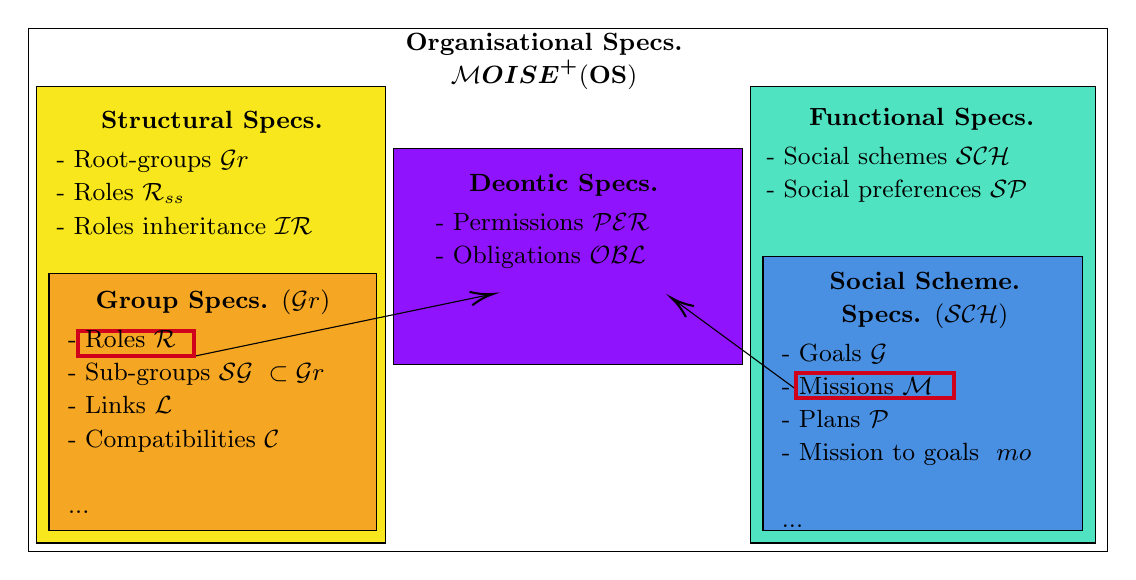
\begin{tikzpicture}[x=0.75pt,y=0.75pt,yscale=-1,xscale=1]
%uncomment if require: \path (0,1656); %set diagram left start at 0, and has height of 1656

%Shape: Rectangle [id:dp6756844921493015] 
\draw  [fill={rgb, 255:red, 248; green, 231; blue, 28 }  ,fill opacity=1 ] (46,1204) -- (214,1204) -- (214,1424) -- (46,1424) -- cycle ;
%Shape: Rectangle [id:dp3759944257810566] 
\draw  [fill={rgb, 255:red, 80; green, 227; blue, 194 }  ,fill opacity=1 ] (390,1204) -- (556,1204) -- (556,1424) -- (390,1424) -- cycle ;
%Shape: Rectangle [id:dp28244406216006945] 
\draw  [fill={rgb, 255:red, 144; green, 19; blue, 254 }  ,fill opacity=1 ] (218,1234) -- (386,1234) -- (386,1338) -- (218,1338) -- cycle ;
%Shape: Rectangle [id:dp32232123359581766] 
\draw   (42,1176) -- (562,1176) -- (562,1428) -- (42,1428) -- cycle ;
%Shape: Rectangle [id:dp7605706269262755] 
\draw  [fill={rgb, 255:red, 74; green, 144; blue, 226 }  ,fill opacity=1 ] (396,1286) -- (550,1286) -- (550,1418) -- (396,1418) -- cycle ;
%Shape: Rectangle [id:dp33110985390647496] 
\draw   (52,1294) -- (210,1294) -- (210,1418) -- (52,1418) -- cycle ;
%Shape: Rectangle [id:dp8653560038381976] 
\draw  [fill={rgb, 255:red, 245; green, 166; blue, 35 }  ,fill opacity=1 ] (52,1294) -- (210,1294) -- (210,1418) -- (52,1418) -- cycle ;
%Straight Lines [id:da09781093164567278] 
\draw    (412,1350) -- (353.61,1307.18) ;
\draw [shift={(352,1306)}, rotate = 36.25] [color={rgb, 255:red, 0; green, 0; blue, 0 }  ][line width=0.75]    (10.93,-3.29) .. controls (6.95,-1.4) and (3.31,-0.3) .. (0,0) .. controls (3.31,0.3) and (6.95,1.4) .. (10.93,3.29)   ;
%Straight Lines [id:da3938396723807833] 
\draw    (122,1334) -- (264.04,1304.41) ;
\draw [shift={(266,1304)}, rotate = 168.23] [color={rgb, 255:red, 0; green, 0; blue, 0 }  ][line width=0.75]    (10.93,-3.29) .. controls (6.95,-1.4) and (3.31,-0.3) .. (0,0) .. controls (3.31,0.3) and (6.95,1.4) .. (10.93,3.29)   ;
%Shape: Rectangle [id:dp269311335478327] 
\draw  [color={rgb, 255:red, 208; green, 2; blue, 27 }  ,draw opacity=1 ][line width=1.5]  (66,1322) -- (122,1322) -- (122,1334) -- (66,1334) -- cycle ;
%Shape: Rectangle [id:dp7449860119164387] 
\draw  [color={rgb, 255:red, 208; green, 2; blue, 27 }  ,draw opacity=1 ][line width=1.5]  (412,1342) -- (488,1342) -- (488,1354) -- (412,1354) -- cycle ;


% Text Node
\draw (472.5,1237.41) node   [align=left] {\begin{minipage}[lt]{112.2pt}\setlength\topsep{0pt}
\begin{center}
\textbf{{\small Functional Specs.}}
\end{center}
{\small  - Social schemes $\displaystyle \mathcal{SCH}$}\\{\small  - Social preferences $\displaystyle \mathcal{SP}$}
\end{minipage}};
% Text Node
\draw (474,1355) node   [align=left] {\begin{minipage}[lt]{103.36pt}\setlength\topsep{0pt}
\begin{center}
\textbf{{\small Social Scheme.}}\\{\small \textbf{Specs. }$\displaystyle (\mathcal{SCH})$}
\end{center}
{\small  - Goals $\displaystyle \mathcal{G}$}\\{\small  - Missions $\displaystyle \mathcal{M}$}\\{\small  - Plans $\displaystyle \mathcal{P}$}\\{\small  - Mission to goals \ $\displaystyle mo$}\\\\{\small  ...}
\end{minipage}};
% Text Node
\draw (131,1356) node   [align=left] {\begin{minipage}[lt]{104.72pt}\setlength\topsep{0pt}
\begin{center}
{\small \textbf{Group Specs. }$\displaystyle (\mathcal{G} r)$}
\end{center}
{\small  - Roles $\displaystyle \mathcal{R}$}\\{\small  - Sub-groups $\displaystyle \mathcal{SG} \ \subset \mathcal{G} r$}\\{\small  - Links $\displaystyle \mathcal{L}$}\\{\small  - Compatibilities $\displaystyle \mathcal{C}$}\\\\{\small  ...}
\end{minipage}};
% Text Node
\draw (181,1177) node [anchor=north west][inner sep=0.75pt]   [align=left] {\begin{minipage}[lt]{162.41pt}\setlength\topsep{0pt}
\begin{center}
{\small \textbf{Organisational Specs. }$\displaystyle \mathcal{M}\boldsymbol{OISE^{+}}$($\displaystyle \mathbf{OS}$)}
\end{center}

\end{minipage}};
% Text Node
\draw (300,1269.09) node   [align=left] {\begin{minipage}[lt]{92.48pt}\setlength\topsep{0pt}
\begin{center}
\textbf{{\small Deontic Specs.}}
\end{center}
{\small  - Permissions $\displaystyle \mathcal{PER}$}\\{\small  - Obligations $\displaystyle \mathcal{OBL}$}
\end{minipage}};
% Text Node
\draw (130.5,1245.69) node   [align=left] {\begin{minipage}[lt]{112.2pt}\setlength\topsep{0pt}
\begin{center}
\textbf{{\small Structural Specs.}}
\end{center}
{\small  - Root-groups $\displaystyle \mathcal{G} r$}\\{\small  - Roles $\displaystyle \mathcal{R}_{ss}$}\\{\small  - Roles inheritance $\displaystyle \mathcal{IR}$}
\end{minipage}};


\end{tikzpicture}
    \caption{A synthetic view of the $\mathcal{M}OISE^+$ model}
    \label{fig:moise_model}
\end{figure}

The $\mathcal{M}OISE^+$ organizational model~\cite{Hubner2007} provides a structured approach to multi-agent organization, facilitating the enforcement of role-based constraints in MARL. As illustrated in \autoref{fig:moise_model}, $\mathcal{M}OISE^+$ consists of three core specifications:

\noindent \textbf{1. Structural Specifications (SS)} define agent relationships and roles within the system:
\begin{equation}
    \mathcal{SS} = \langle \mathcal{R}, \mathcal{IR}, \mathcal{G} \rangle.
\end{equation}
where:
\begin{itemize}
    \item $\mathcal{R}$ is the set of roles.
    \item $\mathcal{IR}$ defines inheritance relationships among roles.
    \item $\mathcal{G}$ is the set of organizational groups.
\end{itemize}

\noindent \textbf{2. Functional Specifications (FS)} describe goal-oriented agent behaviors:
\begin{equation}
    \mathcal{FS} = \langle \mathcal{SCH}, \mathcal{PO} \rangle.
\end{equation}
where:
\begin{itemize}
    \item $\mathcal{SCH}$ structures global goals, missions, and plans.
    \item $\mathcal{PO}$ represents mission preferences and execution priorities.
\end{itemize}

\noindent \textbf{3. Deontic Specifications (DS)} enforce role-based permissions and obligations:
\begin{equation}
    \mathcal{DS} = \langle \mathcal{OBL}, \mathcal{PER} \rangle.
\end{equation}
where:
\begin{itemize}
    \item $\mathcal{OBL}$ denotes mandatory role assignments.
    \item $\mathcal{PER}$ specifies optional role permissions.
\end{itemize}

\subsection{Linking $\mathcal{M}OISE^+$ with MARL}

We introduce **Constraint Guides** to bridge the gap between $\mathcal{M}OISE^+$ and MARL, enabling structured policy learning. These guides enforce agent behavior through modifications to action spaces and rewards.

\noindent \textbf{1. Role Action Guide (RAG)}: Limits action choices based on predefined role constraints:
\begin{equation}
    rag: H \times \Omega \rightarrow \mathcal{P}(A \times \mathbb{R}).
\end{equation}

\noindent \textbf{2. Role Reward Guide (RRG)}: Penalizes deviations from expected role-based behaviors:
\begin{equation}
    rrg: H \times \Omega \times A \rightarrow \mathbb{R}.
\end{equation}

\noindent \textbf{3. Goal Reward Guide (GRG)}: Encourages alignment with predefined goal trajectories:
\begin{equation}
    grg: H \rightarrow \mathbb{R}.
\end{equation}

Additionally, we define \textbf{Linkers} to connect $\mathcal{M}OISE^+$ structures with MARL:
\begin{itemize}
    \item \textbf{Agent to Role} ($ar: \mathcal{A} \to \mathcal{R}$) assigns roles to agents.
    \item \textbf{Role to Constraint Guide} ($rcg: \mathcal{R} \rightarrow rag \cup rrg$) links roles to action and reward constraints.
    \item \textbf{Goal to Constraint Guide} ($gcg: \mathcal{G} \rightarrow grg$) associates goals with reward incentives.
\end{itemize}

\autoref{fig:mm_synthesis} illustrates the overall MOISE+MARL framework, integrating $\mathcal{M}OISE^+$ specifications with constraint-guided MARL training.

\subsection{Solving the MOISE+MARL Problem}

The goal is to find an optimal joint policy $\pi^j$ that maximizes the modified state-value function:
\begin{equation}
    V^{\pi^{j}}(s_t) = \sum_{a_t \in A_t} \pi^j(a_t | \omega_t) \sum_{s_{t+1} \in S} T(s_{t+1} | s_t, a_t) [R' + V^{\pi^{j}}(s_{t+1})].
\end{equation}
where:
\begin{equation}
    R' = R(s_t, a_t, s_{t+1}) + grg(h_t) - rrg(h_t, \omega_t, a_t).
\end{equation}

This formulation ensures that agents **adhere to organizational roles** while optimizing performance in MARL.

\subsection{Implementation Considerations}
Implementing constraint guides manually is tedious. To simplify this, we introduce **Trajectory-based Patterns (TPs)**, inspired by NLP methods, to encode behavioral constraints. A TP $p \in P$ is defined as:
\begin{equation}
    p = \langle h, (c_{\text{min}}, c_{\text{max}}) \rangle.
\end{equation}
where $h$ represents a sequence of observations/actions, and $(c_{\text{min}}, c_{\text{max}})$ defines repetition constraints.

By leveraging these patterns, constraint enforcement becomes more interpretable and scalable. The MOISE+MARL framework enables structured MARL training through the integration of the $\mathcal{M}OISE^+$ organizational model.


\section{The TEMM Method}
\label{sec:TEMM_algorithm}

As presented in \autoref{sec:related_works}, no existing method fully meets our requirements for determining abstract roles, abstract goals, or organizational fit. To address this gap, we propose the \textbf{Trajectory-based Evaluation in MOISE+MARL} (TEMM) method for the automatic inference and evaluation of roles and missions based on observed behaviors over multiple episodes.

\

\noindent TEMM leverages unsupervised learning techniques to generalize abstract roles and missions from observed behaviors across multiple test episodes. By measuring the deviation between inferred abstract organizational specifications and actual agent behaviors, TEMM quantifies \textit{organizational fit}, providing a measure of how well a policy aligns with inferred abstract organizational structures.

\subsection{Formalizing Organizational Inference in TEMM}

TEMM is based on a set of definitions that link $\mathcal{M}OISE^+$ organizational specifications to observed joint histories. Each specification is inferred using dedicated unsupervised learning techniques that progressively build an abstract organization based on agent behaviors.

\noindent The TEMM method follows a three-step process:
\begin{enumerate}
    \item **Inferring roles and their inheritance** using hierarchical clustering.
    \item **Inferring goals, plans, and missions** using trajectory clustering and observation-state analysis.
    \item **Inferring obligations and permissions** by analyzing temporal constraints and goal consistency.
\end{enumerate}

\noindent The following sections detail each of these steps.
%
\footnotetext[1]{ \label{fn:github} Additional details, developed code, datasets, and hyperparameter configurations are available at \url{https://github.com/julien6/MOISE-MARL}.}

\subsection{Inferring Roles and Their Inheritance}

We define a \textbf{role} $\rho$ as a set of policies whose associated agent histories share a \textbf{Common Longest Subsequence (CLS)}. A role $\rho_2$ is considered a \textbf{sub-role} of $\rho_1$ if the CLS of histories associated with $\rho_2$ is contained within that of $\rho_1$. This definition formalizes role abstraction in MARL.

To infer roles, TEMM applies a \textit{hierarchical clustering} algorithm to identify CLSs across agent histories:
\begin{equation}
    \rho = \text{argmax}_{\rho} \left( \sum_{h \in H_{\rho}} | \text{CLS}(h, H_{\rho}) | \right),
\end{equation}
where $\text{CLS}(h, H_{\rho})$ is the longest common sequence among histories in role $\rho$.

A \textbf{dendrogram} representation of clustering results allows for the visualization of inferred hierarchical role structures. Given the hierarchical nature of CLS extraction, TEMM recursively partitions histories into increasingly abstract roles, ensuring organizational coherence.

\noindent **Measuring Structural Organizational Fit:**  
TEMM computes the alignment between agent trajectories and inferred abstract roles:
\begin{equation}
    \text{Structural Fit} = \frac{1}{|H|} \sum_{h \in H} \frac{| \text{CLS}(h, H_{\rho(h)}) |}{|h|}.
\end{equation}

\subsection{Inferring Goals, Plans, and Missions}

A \textbf{goal} is defined as a recurring set of joint observations reached by successful agents following their trajectories. A \textbf{mission} consists of a set of goals collectively achieved by an agent.

To infer goals, TEMM follows these steps:
\begin{enumerate}
    \item Compute a \textbf{joint-observation transition graph} for each joint-history.
    \item Merge transition graphs into a general \textbf{global transition model}.
    \item Cluster observation sequences using \textbf{K-means} to identify trajectory patterns.
    \item Sample key joint-observations as \textbf{abstract goals}.
\end{enumerate}

A goal $g$ is identified as:
\begin{equation}
    g = \text{argmin}_{o \in \Omega} \left( \sum_{h \in H} d_{\text{traj}}(o, H) \right),
\end{equation}
where $d_{\text{traj}}(o, H)$ represents the variance of joint-observations $o$ across all agent trajectories.

Using the inferred goals, TEMM reconstructs \textbf{plans} by identifying sequential dependencies:
\begin{equation}
    p = \{ (g_i, g_j) \ | \ g_j \text{ follows } g_i \text{ in at least } k\% \text{ of episodes} \}.
\end{equation}

A \textbf{mission} is defined as the set of goals pursued by an agent over multiple episodes:
\begin{equation}
    m = \{ g_1, g_2, \dots, g_n \}, \quad \forall g_i \in G, P(m | G) > \theta.
\end{equation}

\noindent **Measuring Functional Organizational Fit:**  
To measure how well a policy conforms to inferred abstract goals:
\begin{equation}
    \text{Functional Fit} = \frac{1}{|H|} \sum_{h \in H} \frac{| g(h) \cap G |}{| G |}.
\end{equation}

\subsection{Inferring Obligations and Permissions}

An \textbf{obligation} exists when an agent, playing role $\rho$, exclusively fulfills the goals of a mission $m$ within a given time frame. A \textbf{permission} is granted when an agent may accomplish other goals outside of its mission.

TEMM determines obligations and permissions by:
\begin{enumerate}
    \item Identifying agent-to-mission associations.
    \item Checking whether an agent's behavior remains within predefined time constraints.
    \item Analyzing deviations from inferred mission structures.
\end{enumerate}

A role $\rho$ is obligated to a mission $m$ if:
\begin{equation}
    \sum_{g \in G_m} P(g | \pi_{\rho}) > \theta_{\text{obligation}}, \quad P(g_{\neg m} | \pi_{\rho}) \approx 0.
\end{equation}
Conversely, a role is permitted to deviate if:
\begin{equation}
    P(g_{\neg m} | \pi_{\rho}) > \theta_{\text{permission}}.
\end{equation}

\noindent **Final Organizational Fit Calculation:**  
\begin{equation}
    \text{Organizational Fit} = \text{Structural Fit} + \text{Functional Fit}.
\end{equation}

\subsection{Manual Refinement and Stability Considerations}

Despite the use of clustering techniques, manual configuration is required to avoid artifacts that may distort the inferred organizational structure. Hyperparameters such as the number of clusters in K-means or the depth of hierarchical clustering must be tuned to balance specificity and generalizability.

Furthermore, TEMM suggests an \textbf{interactive refinement process}:
\begin{itemize}
    \item **Visual inspection of inferred roles and goals.**
    \item **Post-processing techniques to remove noise.**
    \item **User-defined constraints to refine clusters.**
\end{itemize}

While clustering algorithms provide an initial organizational framework, expert intervention is recommended to ensure meaningful abstractions. The TEMM method enables automated inference of structural and functional organization in MARL by extracting abstract roles, goals, and missions from agent behaviors. By defining organizational fit as the sum of structural and functional fit, TEMM provides a quantitative measure of policy alignment with inferred organizational structures.

\section{Experimental framework}
\label{sec:experimental_setup}

This section details the experimental framework used to evaluate the MOISE+MARL framework.% We adapted existing tools to implement our approach. We then present the environments used, the MARL algorithms, the organizational specifications, and the evaluation metrics.

\subsection{Implementing MOISE+MARL}

We have developed an implementation of the MOISE+MARL framework called \textquote{MMA}~\hyperref[fn:github]{\footnotemark[1]} (MOISE+MARL API), which is a Python API that integrates all theoretical sets and relations to minimize user interactions. MMA uses an Object-oriented approach, structuring the $\mathcal{M}OISE^+$ model as nested data classes, with the "Moise" class at the root, enabling users to define organizational specifications, such as roles, goals, and permissions.

To support Dec-POMDP environments, we utilized the \textit{PettingZoo} library \cite{terry2020pettingzoo}, which provides a standard API for multi-agent systems and ensures interoperability across various environments, similar to the Gymnasium framework \cite{kwiatkowski2024}. MMA incorporates a dictionary for observation/action label mapping ($l$), which users can customize, and it also supports Trajectory Patterns (TPs) to facilitate pattern definition and matching.

Each type of constraint guide, like $rag$, $rrg$, and $grg$, is implemented as a separate class. Users can define these guides with custom functions or JSON rules; for example, $rag$ can be instantiated by associating a (TP, last observation) pair with expected actions, while $grg$ can apply bonuses based on specific TPs. The global "MMA" class integrates these guides with user-defined relations, such as linking an agent to a role ($ar$) or associating a role with $rrg$ and $rag$, incorporating the organizational specifications defined in the $\mathcal{M}OISE^+$ structure.

Once set up, the MMA object is used to encapsulate the environment with a \textit{PettingZoo} wrapper. This wrapper applies action masks and modifies rewards at each step, ensuring that agents adhere to the organizational specifications throughout training. MMA also integrates \textit{MARLlib} \cite{hu2021marlib}, which provides access to state-of-the-art MARL algorithms, enabling training to be run on a high-performance computing cluster.

After training, the TEMM method is employed, using manually optimized hyperparameters to infer abstract roles and goals through hierarchical clustering and K-means. This analysis generates visual outputs, such as dendrograms for roles and joint-observation transition graphs for goals. The resulting abstract roles and goals can be exported as JSON trajectories, providing a structured view of the inferred organizational behaviors.


\subsection{Environments used}

We tested our MOISE+MARL framework in four distinct multi-agent environments. These environments were selected for their diversity in terms of collaboration, competition, and resource management. Here is a description of each:

\begin{itemize}
    \item \textbf{Predator-Prey}: A classic environment where several predators must cooperate to capture prey. This environment tests the agents' ability to coordinate their actions to achieve a collective goal\cite{lowe2017multi}

    \item \textbf{Overcooked-AI}: A team cooking game where several agents must collaborate to prepare and serve dishes in increasingly complex kitchens\cite{overcookedai}. Agents must manage tasks such as chopping, cooking, assembling, and serving ingredients while optimizing their movements and avoiding obstacles. This environment is ideal for testing coordination and task allocation in dynamic, highly interdependent scenarios, where clear roles (such as "chef," "assistant," "server") can be defined via organizational specifications
    
    \item \textbf{Warehouse Management}: A proposed environment, where agents must manage a warehouse by coordinating resource deliveries to demand points. Roles and missions here influence agent specialization in specific tasks (transportation of products, inventory management)
    
    \item \textbf{Cyber-Defense Simulation}: A complex environment simulating network defense against cyberattacks. Agents must identify and counter threats while adhering to strict security rules, thus testing the robustness and safety of trained agents\cite{Maxwell2021}.
\end{itemize}

These environments are encapsulable in the PettingZoo API, enabling seamless integration with our MOISE+MARL implementation and facilitating the application of organizational specifications.

\subsection{MARL algorithms used}

We evaluated our framework with several MARL algorithms :
%
% \begin{enumerate*}[label={\roman*)}, itemjoin={; \quad}]
\begin{itemize}
    \item \textbf{MADDPG (Multi-Agent Deep Deterministic Policy Gradient)}~\cite{lowe2017multi}: A centralized learning, decentralized execution algorithm, allowing each agent to have a deterministic policy while using global information during training
    
    \item \textbf{MAPPO (Multi-Agent Proximal Policy Optimization)}~\cite{yu2021mappo}: An adapted version of PPO for MAS, optimized for stable joint policy convergence in complex scenarios
    
    \item \textbf{Q-Mix}~\cite{rashid2018qmix}: A Q-value-based algorithm that learns to combine individual agents' Q-values into a joint value to optimize cooperation
    
    \item \textbf{COMA (Counterfactual Multi-Agent) }~\cite{foerster2018counterfactual} An actor-critic algorithm able to estimate the impact of an individual agent's actions on the team's overall reward.
\end{itemize}
% \end{enumerate*}

\subsection{Organizational specifications}

For each environment, we defined a set of organizational specifications. These specifications include roles, missions, as well as permissions and obligations for each agent. Here, we give an informal description of these~\hyperref[fn:github]{\footnotemark[1]}:
%
\begin{itemize}
    \item \textbf{Predator-Prey}: Predator and prey roles are defined, with each predator having specific objectives such as "capture the prey" or "block escape routes."

    \item \textbf{Overcooked-AI}: Agents adopt three main roles: chef, assistant, and server. The Chef is responsible for cooking and assembling dishes, the Assistant handles ingredient chopping and supply, and the Server is in charge of delivering dishes to customers. Missions primarily involve preparing and serving a certain number of dishes within a given time.
    
    \item \textbf{Warehouse Management}: Agents adopt roles such as "transporter" and "inventory manager," with missions related to managing logistics flows and optimized delivery.
    
    \item \textbf{Cyber-Defense Simulation}: Agents have network defender roles, each with obligations such as intrusion detection or protecting specific drone swarm ad hoc networks.
\end{itemize}

\subsection{Computing resources and hyperparameters}

All experiments were conducted on an academic high-performance computing cluster, utilizing various configurations of GPU nodes. Specifically, we employed nodes equipped with NVIDIA A100 and V100 GPUs, and AMD MI210 GPUs. Each algorithm-environment combination was executed on 5 parallel instances to ensure robust and consistent results. 

Hyperparameters~\hyperref[fn:github]{\footnotemark[1]} for each algorithm, including learning rates, discount factors, and exploration rates, were either retrieved from MARLlib data banks or optimized for each environment through a grid search using the \textit{Optuna} tool~\cite{akiba2019optuna}.

\subsection{Evaluation metrics and protocol}

To measure the effectiveness of the learned policies and the impact of organizational specifications, we defined the following metrics:
%
\begin{enumerate*}[label={\roman*)}, itemjoin={; \quad}]
    \item \textbf{Cumulative Reward}: Measures policy effectiveness in achieving environment goals
    \item \textbf{Reward Standard Deviation}: Reflects the stability of learned policies over episodes
    \item \textbf{Convergence Rate}: Indicates the speed at which policies achieve stable performance
    \item \textbf{Constraint Violation Rate}: Assesses policy adherence to organizational constraints, critical for safety
    \item \textbf{Consistency Score}: Evaluates alignment between trained behaviors and organizational specifications
    \item \textbf{Robustness Score}: Measures agents' ability to maintain performance under a series of challenging scenarios
    \item \textbf{Organizational Fit Level}: Quantifies the organizational fit.
\end{enumerate*}

\

\noindent Our protocol compares the \textit{Reference Baseline} (RB) without organizational constraints and the \textit{Organizationally Constrained Baseline} (OB) using MOISE+MARL.

We use the MMA software to establish the RB with no organizational specifications. For each environment, we train agents with each algorithm until rewards converge or a maximum episode limit is reached. We record metrics and select the algorithm that achieves the highest Cumulative Reward as the RB (control scenario without constraints).
%
For the OB, we reset environments and agents, applying pre-defined organizational specifications using MMA so that each agent is assigned a role. We train these agents with the RB's highest-performing algorithm, again until convergence or the episode limit. After training, we compute all metrics, providing a scenario with organizational constraints as the OB.

By comparing the RB and OB, we can validate the impact of MOISE+MARL on organizational fit. First, we check if the agents' behaviors align with the specified roles in the OB. We analyze manually or rely on reliable metrics like Reward Standard Deviation, Convergence Rate, and Robustness Score. If agents behave in ways that align with their roles, then we favor the idea that MOISE+MARL has influenced organizational fit.
%
Therefore, we should observe differences in the Organizational Fit Level metric between RB and OB. We can also push forward a correlation between fully/freely constraining roles and higher/lower Organizational Fit Level. If all of these observations hold, then the Organizational Fit Level may quantify the organizational fit, and the Consistency Score metric may be used to validate the effectiveness of MOISE+MARL in controlling organizational fit when roles are applied.

Finally, we also check the relevance of the $\mathcal{M}OISE^+$ by comparing MOISE+MARL with its AGR equivalent called AGR+MARL which only considers roles and  does not explicitly include goals.

\section{Results}
\label{sec:results}

This section presents and analyzes the experimental results from applying the MOISE+MARL framework across various environments, highlighting key metrics and comparisons with AGR+MARL.

\begin{figure}
    \centering
    \includegraphics[width=\linewidth]{figures/wm_learning_curve.png}
    \caption{Learning curve for the Warehouse Management environment using IPPO.}
    \label{fig:wm_learning_curve}
\end{figure}

\begin{figure}
    \centering
    \includegraphics[width=0.4\linewidth]{figures/screenshot_1.png}
    \includegraphics[width=0.4\linewidth]{figures/wm_screenshot.png}
    \caption{Screenshot examples from the Warehouse Management environment and Predator Prey environments.}
    \label{fig:env_screenshots}
\end{figure}

\begin{table*}[h!]
    \centering
    \caption{Detailed results for each environment and favored algorithm under both RB and OB.}
    \label{tab:detailed_results}
    \small
    \renewcommand{\arraystretch}{1.2}
    \begin{tabular}{p{2cm}p{1.7cm}p{1.cm}p{1.cm}p{1.cm}p{1.cm}p{1.cm}p{1.7cm}p{1.7cm}p{1.2cm}}
        \hline
        \textbf{Env.} & \textbf{Alg.} & \textbf{Org. Spec.} & \textbf{Cum. Rew.} & \textbf{STD} & \textbf{Conv. Rate} & \textbf{Viol. Rate} & \textbf{Cons. Score} & \textbf{Rob. Score} & \textbf{Org. Fit Lvl} \\ \hline
        Predator-Prey & MADDPG &  & 200.1 & 21.5 & 0.65 & - & - & 0.65 & 0.43 \\
        Predator-Prey & MADDPG & Yes & 245.8 & 15.2 & 0.85 & 5.0\% & 0.81 & 0.83 & 0.87 \\
        Overcooked-AI & MAPPO &  & 348.2 & 15.6 & 0.75 & - & - & 0.71 & 0.48 \\
        Overcooked-AI & MAPPO & Yes & 391.2 & 10.4 & 0.92 & 3.5\% & 0.89 & 0.89 & 0.91 \\
        Warehouse Management & Q-Mix &  & 257.4 & 18.9 & 0.74 & - & - & 0.68 & 0.50 \\
        Warehouse Management & Q-Mix & Yes & 307.1 & 13.8 & 0.88 & 4.2\% & 0.88 & 0.86 & 0.90 \\
        Cyber-Defense & COMA &  & 162.4 & 17.3 & 0.70 & - & - & 0.67 & 0.45 \\
        Cyber-Defense & COMA & Yes & 188.9 & 11.2 & 0.86 & 4.8\% & 0.76 & 0.80 & 0.83 \\ \hline
    \end{tabular}
\end{table*}

\subsection{Quantitative organizational fit and consistency}

Table~\ref{tab:detailed_results} summarizes the performance metrics for each environment and the most efficient algorithm under both the RB and OB. Across all environments, the organizational fit metric is significantly higher under the OB, confirming that MOISE+MARL effectively aligns agent behaviors with organizational specifications.

For example, in the \textbf{Predator-Prey} environment with \textbf{MADDPG}, agents in the OB configuration achieved an organizational fit level of 0.87, which represents a 44\% increase compared to the RB (0.43). Similarly, in the \textbf{Overcooked-AI} environment, \textbf{MAPPO} under the OB reached an organizational fit of 0.91 (an increase of 89\% over the RB's 0.48). These improvements are mirrored in the \textbf{Warehouse Management} environment with \textbf{Q-Mix}, where the organizational fit rose from 0.50 in the RB to 0.90 in the OB, suggesting a MOISE+MARL's consistent effectiveness.

In general, agents constrained with organizational specifications show a lower reward deviation and a higher convergence rate that suggests an impact on their behavior. We manually observed agents' interactions in visualizable environments such as Predator-Prey or Warehouse Management and verified that trained agents' behaviors do align with the expected behavior of a structural and functional abstract organization.
%
Indeed, the significant variation depending on the application of organizational specifications on agents, and the manually verified alignment of agents with roles suggests that organisational fit level correlates with the organizational fit.

Considering organizational fit level reliable across all environments, the \textbf{consistency score} also shows important values with a minimal value of 0.76 for the \textbf{Cyber-Defense} environment. This suggests that despite a noisy environment that introduces some disturbance in agents' behavior, the inferred organizational specifications are still close to applied ones.

\subsection{Performance and stability across algorithms}

The results indicate that policy-based and actor-critic algorithms like \textbf{MADDPG} and \textbf{MAPPO} benefit substantially from the MOISE+ MARL framework, particularly in terms of consistency and stability. For example, \textbf{MAPPO} in the \textbf{Overcooked-AI} environment saw a reward standard deviation reduction from 15.6 (RB) to 10.4 (OB), reflecting a more stable policy with less behavioral fluctuation. \textbf{MADDPG} in \textbf{Predator-Prey} also showed a similar pattern, with a standard deviation drop from 21.5 in the RB to 15.2 in the OB, indicating increased reliability.

In contrast, value-based algorithms like \textbf{Q-Mix} maintained high performance in cumulative reward but displayed greater variability in consistency. For instance, in \textbf{Warehouse Management}, \textbf{Q-Mix} achieved a reward standard deviation of 13.8 in the OB, a notable improvement over 18.9 in the RB but still higher than the stability observed in policy-based algorithms. This suggests that while \textbf{Q-Mix} is effective for achieving task goals, it may require further tuning for roles with MOISE+MARL to enhance consistency.

\subsection{Impact of organizational constraints on policy convergence, robustness and violation rates}

Applying organizational constraints resulted in faster convergence rates across all environments. In the \textbf{Cyber-Defense} environment, \textbf{COMA} with MOISE+MARL converged at a rate of 0.86, compared to 0.70 in the RB. Similar trends were observed in the \textbf{Warehouse Management} environment with \textbf{Q-Mix}, which showed an improvement from 0.74 in the RB to 0.88 in the OB. This expedited convergence can be attributed to the structured guidance of roles and missions, which narrows the policy search space.

In addition to the presented results where constraint hardness is set to 1, we observed that constraint violation rates were consistently higher when organizational constraints were defined with a lower constraint hardness. In \textbf{Overcooked-AI}, \textbf{MAPPO} recorded a violation rate of 3.5\% with a constraint hardness of 1, compared to 7.1\% with a constraint hardness of 0. Similarly, in \textbf{Warehouse Management}, \textbf{Q-Mix} reduced the violation rate from 7.8\% to 4.2\% as constraint hardness increased. This further supports the framework's effectiveness in enhancing adherence to desired behaviors.

Additionally, we observed a consistent improvement in robustness when organizational specifications were applied to agents. For instance, \textbf{MADDPG} in \textbf{Predator-Prey} and \textbf{MAPPO} in \textbf{Overcooked-AI} achieved high consistency scores of 0.81 and 0.89, respectively, indicating that agents closely followed the inferred roles. Robustness also improved, with \textbf{MAPPO} in \textbf{Overcooked-AI} achieving a robustness score of 0.89, up from 0.71 in the RB, underscoring the framework's impact on agents' resilience to perturbations.

However, one can point out a potential bias: organizational specifications were specifically designed to encompass all observations, avoiding new situations that agents may not be able to handle.


\subsection{Comparison between MOISE+MARL and AGR+MARL}

\begin{table}[h!]
    \centering
    \caption{Performance comparison between MOISE+MARL and AGR+MARL.}
    \label{tab:ablation_study}
    \small
    \renewcommand{\arraystretch}{1.1}
    \begin{tabular}{p{1.6cm}p{0.5cm}p{0.6cm}p{1.4cm}p{0.8cm}p{1.3cm}}
        \hline
        \textbf{Framework} & \textbf{Env.} & \textbf{Conv. Rate} & \textbf{Robustness Score} & \textbf{Org. Fit} & \textbf{Cumulative Reward} \\ \hline
        MOISE+MARL & PP & 0.85 & 0.83 & 0.87 & 245.8 \\
        AGR+MARL & PP & 0.75 & 0.69 & 0.56 & 208.4 \\
        MOISE+MARL & OA & 0.92 & 0.89 & 0.91 & 391.2 \\
        AGR+MARL & OA & 0.82 & 0.75 & 0.58 & 348.9 \\
        MOISE+MARL & WM & 0.88 & 0.86 & 0.90 & 307.1 \\
        AGR+MARL & WM & 0.76 & 0.72 & 0.61 & 278.6 \\ \hline
    \end{tabular}
\end{table}

\noindent Table~\ref{tab:ablation_study} highlights the impact of intermediary goals within MOISE+ MARL compared to AGR+MARL, which only utilizes roles. In \textbf{Overcooked-AI}, \textbf{MAPPO} under MOISE+MARL achieved a cumulative reward of 391.2, with an organizational fit of 0.91—33\% higher than AGR+MARL's 0.58. Similarly, in \textbf{Warehouse Management}, \textbf{Q-Mix} under MOISE+MARL attained a cumulative reward of 307.1, an increase of nearly 10\% over AGR+MARL's 278.6, with a higher robustness score (0.86 vs. 0.72).

Overall, these results underscore the importance of intermediary goals in fostering more stable, goal-oriented behaviors. By facilitating a clearer path to the global objective, MOISE+MARL consistently outperforms AGR+MARL in achieving higher rewards, robustness, and organizational fit across Predator-Prey (PP), Warehouse Management (WM), and Overcooked-AI (OA).


\section{Conclusion and future works}
\label{sec:discussion_conclusion_future_work}

The MOISE+MARL framework introduced in this paper aims to enhance control and explainability in MARL by incorporating organizational models that define explicit roles and missions for agents. Experimental results across several environments indicate that this framework helps agents adhere to expected behaviors while facilitating better policy convergence by constraining the policy search space. The results also show that agents trained with roles and goals exhibit behaviors closely resembling those determined via the framework, suggesting coherence between the application of organizational specifications and their expected posterior effects.

However, the framework's reliance on predefined organizational specifications means it may struggle to adapt in highly dynamic or unstructured environments where agent roles and missions are less defined or evolve over time.
Moreover, the computational overhead associated with enforcing organizational constraints and dynamically modifying rewards and actions may pose scalability challenges. Additionally, TEMM can be computationally intensive, which may hinder its applicability in real-time scenarios or environments with a large number of agents.

We are currently pursuing three main directions for future research:
%
\begin{enumerate*}[label={\roman*)}, itemjoin={; \quad}]
% \begin{enumerate}
    \item Developing adaptive mechanisms that allow roles and missions to evolve dynamically during training could enhance the framework's flexibility, enabling agents to respond to changes in real-time
    \item Exploring automated methods, such as Large Language Models, for generating organizational specifications based on observed agent behaviors to help users on defining these specifications manually
    \item Improving the computational efficiency of TEMM or exploring alternative evaluation methods could make the framework more practical for real-world applications with larger agent populations.
\end{enumerate*}


\section*{References}

% \bibliographystyle{abbrv}
\bibliographystyle{IEEEtran}
\renewcommand
\refname{}
\bibliography{references}

\end{document}
